\chapter{Results, Discussion and Future work}

\section{SEcubeWallet weaknesses}
In this section, the weaknesses of the SEcubeWallet application are discussed, as well as some ideas about how to fix them.


\subsection{First table corruption}
As explained in session \ref{sec:savewalletaction}, during the application development it was impossible to find the origin (and solution) to an error concerning the database saving and opening process: the first table in a wallet is always corrupt. The problem is not present when using the regular SQLite API; it only appears when using the secured version. This seems to point out the error is the secureSQLite library's fault. But because the secureSQLiteBrowser application does not have this problem it is not possible to discard SEcubeWallet as the origin of the problem.

The secureSQLiteBrowser and SEcubeWallet applications differ in the way they use the secureSQLite API. secureSQLiteBrowser, as it is a data base manager, uses complex SQLite functionalities like save points and pragma statements to exploit all of the API's capabilities, while SEcubeWallet only uses simple open/exec/close SQLite functions. So in a way SEcubeWallet is responsible for the error that could be avoided by using more complex SQLite statements. But the secureSQLite library should behave as the regular SQLite API, specially in the most simple cases.

In any case, the implemented workaround in SEcubeWallet (always having an unused and empty first table to sacrifice) should be considered temporary, not only because it is not optimal, but more importantly, because the unfixed error may cause other problems in the future.

\subsection{The FAT32 bug}

Even if the FAT32 bug (see section \ref{sec:fat32bug}) can be considered to be fixed, the truth is its origin is not completely clear, and it may be the case the adopted solution (casting to int) only works for a subset of cases.

\subsection{Only Linux has been tested}

The SEcubeWallet application has only been tested running on Linux. Although Qt is platform independent, some of the application functionalities may need some changes to work on Windows or Mac systems. For example, the zxcvbn compilation process relies on gcc commands, that may not be available in Windows. Moreover the FAT32 bug is a very OS specific issue, as it involves the use of the lseek() function (Linux and Mac). It may be the case the bug does not exists in a Windows machine, or on the contrary there are other errors waiting to be fixed.


\subsection{Missing icons}
The reader of this thesis may have noticed the lack of icons in all of the SEcubeWallet Windows. Due to tight time constraints, it was decided to allocate most of the efforts into other aspects of the application, but that is not to say icons are not important. Future version of the application will definitely have icons to increase the user experience.


\section{Future work}
In this section, a few ideas about how to extend the SEcubeWallet functionalities are given. None of them were considered for this work as they are either too time consuming to implement, or are out of the author's expertise.


\subsection{SEkey integration}

SEkey is a new library currently under development at Politecnico di Torino by 	Mateus Françani as his master thesis work. The library will sit next to SEfile and SElink, as depicted in Figure \ref{fig:sekey} taken from \cite{sekey}.

\begin{figure}[htb]
  \centering
  \captionsetup{justification=centering}
  \centerline{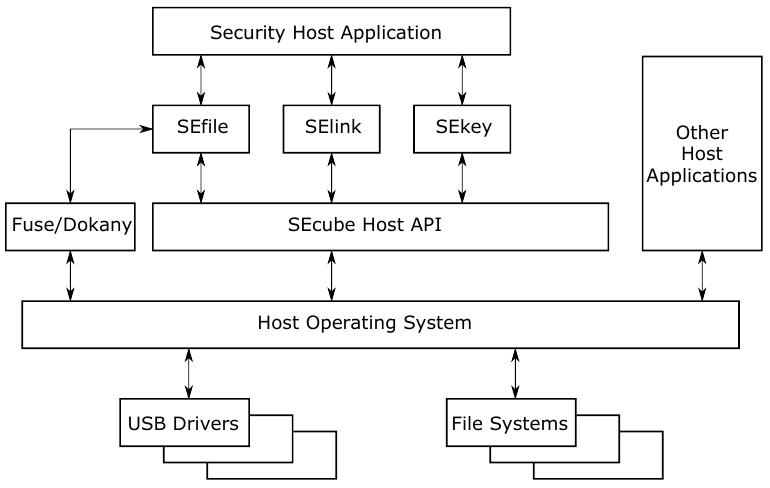
\includegraphics[width=0.8\columnwidth]{chapters/figures/results/sekey.png}}
  \caption{Host side SEcube™ architecture, including the SEkey library}
  \label{fig:sekey}
\end{figure}

The library will work as a key management system for the SEcube™ framework. Right now keys inside a SEcube™ chip can only be modified at factory reset. This is not very useful in a working environment, as the purpose of having multiple keys is to allow users to share information with selected people (people sharing a key are known as a group). The job of the SEkey library will be to allow an administrator to dynamically add and remove keys to SEcube™ devices using an intuitive GUI. By doing so, the administrator can conform groups of users, that later on can use their SEcube™ devices to share sensitive information, knowing it will be secured against unauthorized access (from people outside the group).

As the SEcubeWallet application already offers an intuitive GUI for the management of passwords, it could be extended to support the management of keys as well. If the person login in is an administrator, the application should offer the possibility to edit the keys present in the SEcube™ device. If it is a regular user, it should only let them see what keys they can use, i.e. to which groups they belong.

\subsection{Browser integration} 

The vast majority of users store their internet passwords within their preferred web browser, alongside other sensitive information like browsing history and bookmarks. This allows them to use their passwords easily and fast, as they can for example autofill login credentials in websites.

Exploit the capabilities of the SEcube™ platform to protect all that information while maintaining ease of use and transparency to the final user would be a great advance in the purpose of reaching as many users as possible.

A couple of alternatives come to mind in order to implement this integration:
\begin{itemize}
\setlength\itemsep{-3pt}

\item Borrow the idea followed by the Mooltipass system, porting the entire Qt application to a complement for the most popular web browsers (Firefox, Chrome, Opera).
\item Implement a web browser complement that "talks" with the SecubeWallet application and request for passwords when the user wishes to autofill a login field.
\item Follow the auto-type approach used by the software password manager KeePass. \cite{autotype}. ``KeePass features an "Auto-Type" functionality. This feature allows you to define a sequence of keypresses, which KeePass can automatically perform for you. The simulated keypresses can be sent to any other currently open window of your choice (browser windows, login dialogs, ...). By default, the sent keystroke sequence is \{\textsc{username}\} \{\textsc{tab}\} \{\textsc{password}\} \{\textsc{enter}\}, i.e. it first types the user name of the selected entry, then presses the Tab key, then types the password of the entry and finally presses the Enter key.''
\end{itemize}

In either case ensuring the new functionalities do not compromise the security of the passwords must be the top priority.

\subsection{Mobile application (Android)}
To have a functional SEcubeWallet for the Android system, three elements would need to be ported:
\begin{itemize}
\item The SEcube™ chip. As far as the author knows, the Blu5 group is working on a product that would allow to use the SEcube™ hardware platform in smartphones running the Android OS.
\item The software libraries. The SEfile and secureSQLite libraries are written to work on Linux, Windows and Mac systems. Given that Android is based on Linux, porting the libraries should be possible.
\item The GUI. Qt for Android \cite{android} ``allows to run Qt 5 applications on devices with Android v4.1 (API level 16) or later''. All of the Qt modules used by SEcubeWallet are supported, but a GUI redesign is required in order to cope with the constraints imposed by a smaller display.
\end{itemize}


\subsection{Custom columns}

Wallets in the SEcubeWallet application have a fixed set of columns (\textsc{username}, \textsc{domain}, \textsc{password}, \textsc{description}, \textsc{date}). This set should be enough in most of the cases as they are the standard for wallet managers, but some users may want to add other custom columns, for instance to store "security questions and answers" used by some websites, an email associated to the account, or multiple passwords in the same entry.

\subsection{Expired passwords notification}

Changing passwords regularly is important to keep a high level of security in any system. If the user has a large number of passwords it may be hard to remember when one of them needs to be updated. SEcubeWallet already offers the possibility to search for passwords older than a given period of time (for example passwords older than six months). This functionality could be extended to notify the user when a password needs to be updated. The user could configure the expiration time for each password individually, or for all of them, and how they wish to be notified (Message inside the application, desktop notification, email, etc)






